
\section{Cange detection: strategie}
Il meccanismo di change detection può avvenire in due principali strategie
\begin{itemize}
    \item Default
    \item OnPush
\end{itemize}
La libreria angular adotta la modalità default, che lancia il meccanismo di change detection ogni volta che viene lanciato un evento di interazione con l'utente, questo può portare a cali di prestazione soprattutto con alberi di componenti molto vasti.
È possibile modificare la strategia di change detection utilizzata all'interno della diretiva Compontent
\begin{minted}{typescript}
    @Component({    selector: 'hero-card',    
    changeDetection: ChangeDetectionStrategy.OnPush,    
    template: ...
    })
    export class HeroCard {    ...}
\end{minted}
I componenti che sfruttano la strategia onPush vengono aggiornati solo nei seguenti casi
\begin{itemize}
    \item Vengono modificati i riferimenti delle proprietà utilizzate nel template
    \item Viene lanciato un evento dal componente o da uno dei suoi figli 
    \item Un oggetto osservabile collegato al template emette un nuovo evento
    \item La change detection viene attivata manualmente
\end{itemize}

\begin{figure}[H]
    \centering
 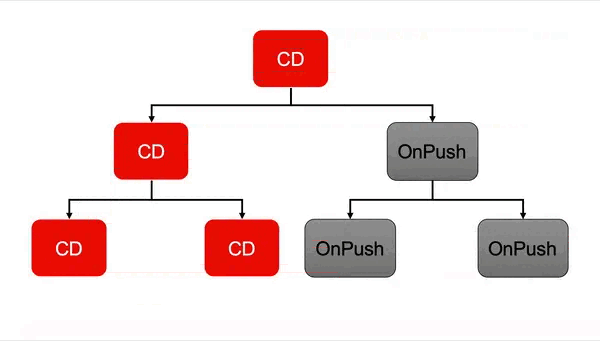
\includegraphics[scale=0.75]{resources/cd-onPush.png}
   \caption{Ciclo di change detection con componenti che sfruttano la strategia onPush}
\end{figure}
In questo modo è possibile evitare che il meccanismo di change detection venga eseguito su componenti di cui non è necessario effettuare sempre l'aggiornamento e rendere l'applicazione più responsiva.
\newline
La strategia onPush tuttavia prevede alcune accortezze per essere utilizzata correttamente. Per come è strutturata la strategia è necessario fornire al template una nuova istanza delle proprietà per poter attivare il meccanismo invece di modificare i valori associati alle proprieta.
\newline
Tuttavia gli oggetti javascript nascono come oggetti mutabili, questo comportamento del linguaggio facilita il manifestarsi di comportamenti non voluti da parte del meccanismo di Change dectection, è consigliabile quindi utilizzare librerie javascript che forniscano oggetti immutabili, come per esempio Immutable.js